\documentclass[tikz]{standalone}
\usepackage{amssymb,dsfont}
\usepackage{color}
\usetikzlibrary{arrows}
% Sets
\newcommand{\CC}{\mathbb{C}}        % Complex numbers
\newcommand{\NN}{\mathbb{N}}        % Natural numbers
\newcommand{\RR}{\mathbb{R}}        % Real numbers
\newcommand{\ZZ}{\mathbb{Z}}        % Relative integers
% Groups
\newcommand{\SO}{\mathrm{SO}}       % Special orthogonal group
\newcommand{\OO}{\mathrm{O}}        % Orthogonal group
\newcommand{\SU}{\mathrm{SU}}       % Special unitary group
\newcommand{\1}{\mathds{1}}		    % trivial group
\newcommand{\DD}{\mathbb{D}}        % Dihedral group
\newcommand{\octa}{\mathbb{O}}      % Cubic (octahedral) group
\newcommand{\ico}{\mathbb{I}}       % Icosahedral group
\newcommand{\tetra}{\mathbb{T}}     % tetrahedral group
\begin{document}
	
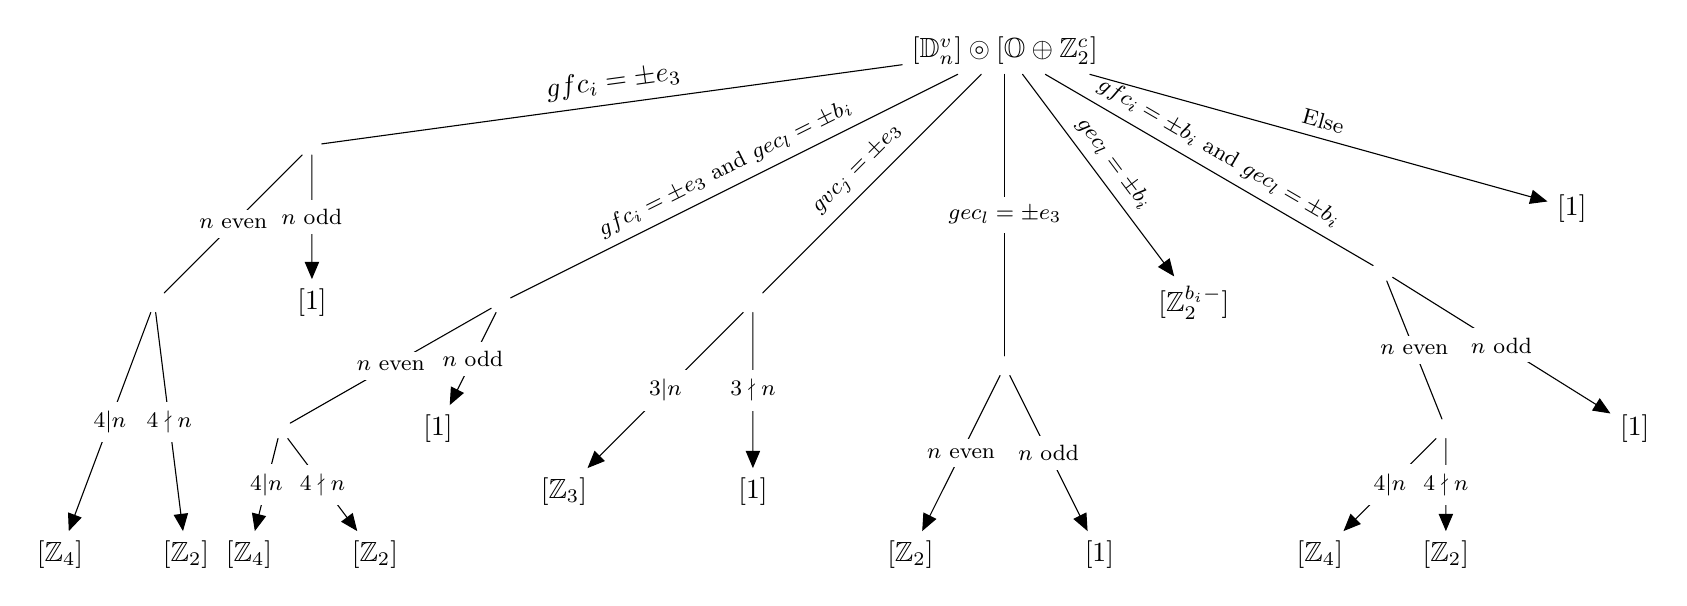
\begin{tikzpicture}[scale=0.8,line cap=round,line join=round,>=triangle 45,x=1.0cm,y=1.0cm]
  \node (root) at (0,0) {$[\DD_n^v]\circledcirc [\octa\oplus \ZZ_2^c]$};

  \node (Bas1) at (-11,-1.5)  {};
  \node (Bas2) at (-8,-4)   {};
  \node (Bas3) at (-4,-4)   {};
  \node (Bas4) at (0,-5)   {};
  \node (Bas5) at (3,-4)    {[$\ZZ_2^{b_i-}]$};   
  \node (Bas6) at (6,-3.5)    {}; 
  \node (Bas7) at (9,-2.5) {$[\1]$};
  \draw (root) -- (Bas1) node [midway,above,sloped] {{ $gfc_i=\pm e_3$ }};
  \draw (root) -- (Bas2) node [midway,above,sloped] {{\footnotesize  $gfc_i=\pm e_3$ and $gec_l=\pm b_i$}};
  \draw (root) -- (Bas3) node [midway,above,sloped] {{\footnotesize  $gvc_j=\pm e_3$}};
  \draw (root) -- (Bas4) node [midway,fill=white] {{\footnotesize  $gec_l=\pm e_3$}};
  \draw[->] (root) -- (Bas5) node [midway,above,sloped] {{\footnotesize  $gec_l=\pm b_i$}};
  \draw (root) -- (Bas6) node [midway,above,sloped] {{\footnotesize $gfc_i=\pm b_i$ and $gec_l=\pm b_i$}};
  \draw[->] (root) -- (Bas7) node [midway,above,sloped] {{\footnotesize  Else}};
  \node (Bas11) at (-11-2.5,-4) {};
  \node (Bas12) at (-11,-4) {$[\1]$};
  \draw (Bas1) -- (Bas11) node [midway,fill=white] {{\footnotesize  $n$ even}};
  \draw[->] (Bas1) -- (Bas12) node [midway,fill=white] {{\footnotesize  $n$ odd}};
  \node (Bas111) at (-13.5-1.5,-8) {[$\ZZ_4$]};
  \node (Bas112) at (-13,-8) {$[\ZZ_2]$};
  \draw [->] (Bas11) -- (Bas111) node [midway,fill=white] {{\footnotesize  $4|n$}};
  \draw [->] (Bas11) -- (Bas112) node [midway,fill=white] {{\footnotesize  $4\nmid n$}};
  \node (Bas21) at (-10-1.5,-6) {};
  \node (Bas22) at (-10+1,-6) {$[\1]$};
  \draw (Bas2) -- (Bas21) node [midway,fill=white] {{\footnotesize  $n$ even}};
  \draw[->] (Bas2) -- (Bas22) node [midway,fill=white] {{\footnotesize  $n$ odd}};
  \node (Bas221) at (-10.5-1.5,-8) {[$\ZZ_4$]};
  \node (Bas222) at (-10.5+0.5,-8) {$[\ZZ_2]$};
  \draw [->] (Bas21) -- (Bas221) node [midway,fill=white] {{\footnotesize  $4|n$}};
  \draw [->] (Bas21) -- (Bas222) node [midway,fill=white] {{\footnotesize  $4\nmid n$}};
  \node (Bas31) at (-4-3,-7) {$[\ZZ_3]$};
  \node (Bas32) at (-4,-7)  {$[\1]$};
  \draw[->] (Bas3) -- (Bas31) node [midway,fill=white] {{\footnotesize  $3|n$}};
  \draw[->] (Bas3) -- (Bas32) node [midway,fill=white] {{\footnotesize  $3\nmid n$}};
  \node (Bas41) at (-1.5,-8) {$[\ZZ_2]$};
  \node (Bas42) at (1.5,-8)  {$[\1]$};
  \draw[->] (Bas4) -- (Bas41) node [midway,fill=white] {{\footnotesize  $n$ even}};
  \draw[->] (Bas4) -- (Bas42) node [midway,fill=white] {{\footnotesize  $n$ odd}};
  \node (Bas61) at (8.5-1.5,-6) {};
  \node (Bas62) at (8.5+1.5,-6) {$[\1]$};
  \draw (Bas6) -- (Bas61) node [midway,fill=white] {{\footnotesize  $n$ even}};
  \draw[->] (Bas6) -- (Bas62) node [midway,fill=white] {{\footnotesize  $n$ odd}};
  \node (Bas661) at (6-1,-8) {[$\ZZ_4$]};
  \node (Bas662) at (6+1,-8) {$[\ZZ_2]$};
  \draw [->] (Bas61) -- (Bas661) node [midway,fill=white] {{\footnotesize  $4|n$}};
  \draw [->] (Bas61) -- (Bas662) node [midway,fill=white] {{\footnotesize  $4\nmid n$}};
\end{tikzpicture}
% Further ’tikzpicture’ environments are possible which will create further pages.
\end{document} 